\documentclass{article}
\usepackage[utf8]{inputenc}
\usepackage[T1]{fontenc}
\usepackage[spanish,mexico]{babel}
\usepackage{graphicx}
\usepackage[a4paper,margin=2.5cm]{geometry}
\usepackage{lmodern}
\usepackage{ragged2e}
\usepackage{array}
\usepackage{tabularx}


\begin{document}
\thispagestyle{empty}

\begin{center}

\includegraphics[width=1\textwidth]{encabezado_utvam.png}
\vspace{0.3cm}
{\small CÁLCULO IV}
\end{center}

\vspace{3cm}
\begin{center}
{\Large \textbf{Coordenadas Polares y Cartesianas}}
\end{center}

\vspace{2.5cm}
\begin{center}
{\Large {Taller de Investigación Pre-Cálculo: Dominando las Coordenadas Polares}}
\end{center}

\vspace{3cm}
\begin{center}
{\small \textbf{INTEGRANTES DEL EQUIPO:}}
\end{center}

\vspace{0.1cm}
\begin{center}
{\small 253110061 - López Lemus Glynnes Eileen}
\end{center}

\vspace{0.1cm}
\begin{center}
{\small 253110509 - Rodriguez Martinez Carlos Eduardo}
\end{center}

\vspace{1cm}
\begin{center}
{\small \textbf{GRUPO: TID-401}}
\end{center}

\vspace{0.1cm}
\begin{center}
{\small \textbf{Docente: Rubén Ramírez Gómez}}
\end{center}

\vfill
\begin{flushright}
{\small OCTUBRE, 2026}
\end{flushright}

\newpage

\begin{justfy}
\small \textbf{1. Definición y Representación Grafica.}

\vspace{0.1cm}
\small {¿Qué es el polo y qué es el eje polar?}

\vspace{0.1cm}
\small {\textbf{- Polo: }Es un punto fijo en el plano que sirve como referencia principal, equivalente al origen (0,0) en el plano cartesiano. A partir de este punto se miden las distancias.}

\vspace{0.1cm}
\small {\textbf{- Eje Polar: }Es un rayo horizontal dirigido hacia la derecha que parte desde el polo, el cual equivale al semieje positivo de las x.}

\vspace{0.3cm}
\small \textbf {Dibujo de las coordenadas:}\[
P_1\left(3,\frac{\pi}{4}\right), \quad
P_2(2,\pi) \text{ y }
P_3\left(4,\frac{3\pi}{2}\right).
\]

\begin{center}
    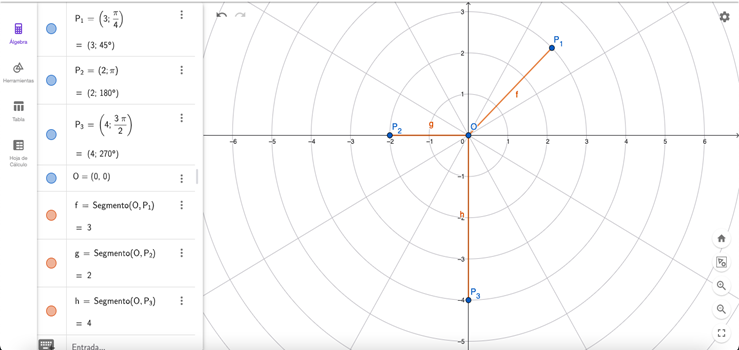
\includegraphics[width=0.9\textwidth]{dibujo_de_puntos.png}
\end{center}

\vspace{0.1cm}
\small {En el plano cartesiano un punto solo tiene un nombre (x,y), pero en coordenadas polares un mismo punto se puede escribir de infinitas formas diferentes. Esto pasa por dos razones muy sencillas:}

\vspace{0.1cm}
\small {1. Dar vueltas completas: Si estás en un punto y das una vuelta completa terminas exactamente en el mismo lugar. Puedes dar las vueltas que quieras y la posición no cambia.}

\vspace{0.1cm}
\small {2. Caminar hacia atrás (radio negativo): Si el radio es negativo no significa que la distancia sea negativa, sino que en lugar de caminar hacia adelante en la dirección del ángulo, caminas hacia atrás en sentido contrario.}

\vspace{0.3cm}
\small \textbf{2. El puente matemático (Conversiones)}

\begin{itemize}
\item \textbf{Hipotenusa ($r$):} Distancia desde el origen al punto.
\item \textbf{Cateto adyacente ($x$):} Distancia horizontal sobre el eje $X$.
\item \textbf{Cateto opuesto ($y$):} Distancia vertical sobre el eje $Y$.
\item \textbf{Ángulo ($\theta$):} Inclinación medida desde el eje polar.
\end{itemize}

\vspace{0.2cm}
\small \textbf {A) Hacia Cartesianas}

Si conocemos $r$ y $\theta$, calculamos $x$ e $y$.

\vspace{0.2cm}
\begin{itemize}
\item {Coordenada $x$:}
\[\cos(\theta)=\frac{x}{r}\]
Despejamos $x$:
\[x=r\cos(\theta)\]

\item {Coordenada $y$:}
\[\sin(\theta)=\frac{y}{r}\]
Despejamos $y$:
\[y=r\sin(\theta)\]
\end{itemize}

\newpage

\small \textbf{B) Hacia Polares}

Si conocemos $x$ e $y$, calculamos $r$ y $\theta$.

\begin{itemize}
\item {Distancia al origen ($r$):}
\[r^2=x^2+y^2\]
Por lo tanto:
\[r=\sqrt{x^2+y^2}\]

\item {Angulo ($\theta$):}
\[\tan(\theta)=\frac{y}{x}\]
Despejamos el angulo:
\[\theta=\arctan\left(\frac{y}{x}\right)\]
\end{itemize}

\vspace{0.3cm}
\small{Identidad clave para limites}
\[x^2+y^2=r^2\]

\vspace{0.3cm}
\small{Demostracion paso a paso}
\[x=r\cos(\theta)\]
\[y=r\sin(\theta)\]

\[x^2+y^2=(r\cos\theta)^2+(r\sin\theta)^2\]
\[x^2+y^2=r^2\cos^2\theta+r^2\sin^2\theta\]
\[x^2+y^2=r^2(\cos^2\theta+\sin^2\theta)\]

\vspace{0.1cm}
\small {Como por identidad trigonométrica $\cos^2 θ+ \sin^2 θ=1,$ la expresión se reduce a:}

\[x^2+y^2=r^2(1)\]

\vspace{0.1cm}
\begin{center}
    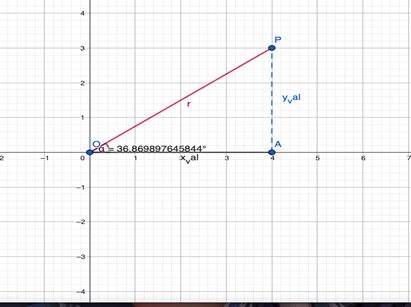
\includegraphics[width=0.7\textwidth]{trigonometria.png}
\end{center}

\vspace{0.1cm}
\small \textbf {3. Visualizacion de Ecuaciones}

\small {A) Ecuacion $r=5$}

\small {Se forma una circunferencia centrada en el origen con un radio de 5 unidades.}

\vspace{0.2cm}
\small {B) Ecuacion $\theta=\frac{\pi}{4}$}

\small {Se forma una recta que pasa por el origen y forma un angulo de 45 grados respecto al eje polar.}

\newpage

\begin{center}
    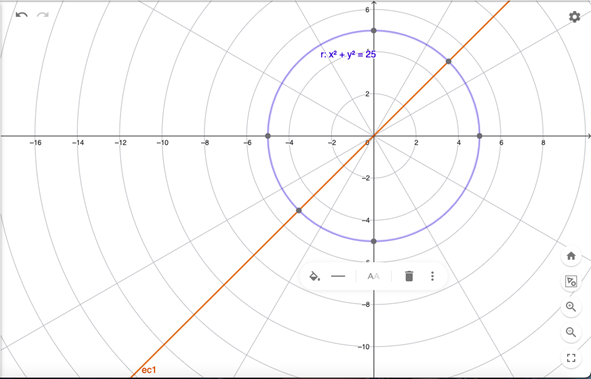
\includegraphics[width=0.8\textwidth]{expresion_original.png}
\end{center}

\small {Expresion original:}

\[\frac{x^2+y^2}{x^2}\]

\small {Para transformar esta expresión completamente a coordenadas polares, aplicamos las relaciones de conversión $x^2+y^2=r^2$ y $x=r⋅\cos(\theta)$:}

\vspace{0.2cm}
\small {Sustitucion de las identidades}

\[\frac{x^2+y^2}{x^2}=\frac{r^2}{(r\cos\theta)^2}\]

\vspace{0.1cm}
\small {Desarrollo del denominador}

\[=\frac{r^2}{r^2\cos^2\theta}\]

\vspace{0.1cm}
\small {Simplificacion del radio }

\[=\frac{1}{\cos^2\theta}\]

\vspace{0.1cm}
\small{Uso de la identidad reciproca}

\[\frac{1}{\cos^2\theta}=\sec^2\theta\]

\small {Resultado final: La expresión expresada totalmente en coordenadas polares equivale a: }

\[\boxed{\sec^2\theta}\]

\vspace{0.3cm}
\small \textbf{4. El concepto de Limite al Origen}

Simplificar el calculo de un limite de varias variables cuando $(x,y)\to(0,0)$ mediante la sustitución a coordenadas polares:

\[x=r\cos(\theta)\]
\[y=r\sin(\theta)\]

\small \textbf {Reducir el limite.}

\small {Reducir la aproximacion al origen $(0,0)$ a la sola condicion de que
el radio tienda a cero $(r\to 0)$, independientemente de la trayectoria
del angulo $\theta$:}

\[\lim_{(x,y)\to(0,0)}f(x,y)=\lim_{r\to0}f(r\cos\theta,r\sin\theta)\]

\newpage

\small \textbf {Criterio de Existencia del Limite}

Analizar la presencia de la variable $\theta$ al evaluar la expresion
resultante:

\begin{enumerate}
\item Determinar la existencia del limite:

\small {Obtener un valor numerico fijo $L$ independiente de $\theta$. Confirmar la existencia del limite global con valor $L$.}

\item Determinar la no existencia del limite:

\small {Obtener un resultado en funcion de $\theta$. Confirmar la no
existencia del limite por variar segun la trayectoria de aproximacion.}
\end{enumerate}

\vspace{0.1cm}
\small \textbf {Demostracion Teorica}

\small {Evaluar el siguiente limite de varias variables:}

\[\lim_{(x,y)\to(0,0)}\frac{x^2y}{x^2+y^2}\]

\begin{enumerate}
\item Sustituir variables:

\small {Aplicar $x=r\cos\theta$, $y=r\sin\theta$ y la identidad
$x^2+y^2=r^2$:}

\[\lim_{r\to 0}\frac{(r\cos\theta)^2(r\sin\theta)}{r^2}\]

\item Desarrollar el numerador:

\[\lim_{r\to 0}\frac{r^3\cos^2\theta\sin\theta}{r^2}\]

\item Simplificar terminos:

\[\lim_{r\to 0}r\cos^2\theta\sin\theta\]

\item Evaluacion de la tendencia:

\small {Sustituir $r=0$:}

\[0\cdot(\cos^2\theta\sin\theta)=0\]

\item Concluir la existencia:

\small {Obtener un resultado constante de $0$ sin dependencia de
$\theta$. Confirmar que el limite existe y es igual a $0$.}
\end{enumerate}

\vspace{0.2cm}
\small \textbf {5. Formulario}

\small {4 formulas de conversion}

\vspace{0.2cm}
\small {Polar a Cartesiana: Conociendo $(r,\theta)$, obtener $x$}

\[x=r\cdot\cos(\theta)\]

\small {Polar a Cartesiana: Conociendo $(r,\theta)$, obtener $y$}

\[y=r\cdot\sin(\theta)\]

\small {Cartesiana a Polar: Conociendo $(x,y)$, obtener $r$}

\[r=\sqrt{x^2+y^2}\]

\small {Cartesiana a Polar: Conociendo $(x,y)$, obtener $\theta$}

\[\theta=\arctan\left(\frac{y}{x}\right)\]

\small \textbf{Identidades Fundamentales}

\begin{enumerate}

\item Relacion Pitagorica:

\[x^2+y^2=r^2\]

\item Identidad Trigonometrica:

\[\cos^2(\theta)+\sin^2(\theta)=1\]

\item Pendiente de la Tangente / Angulo:

\[\tan(\theta)=\frac{y}{x}\quad (x\neq 0)\]

\end{enumerate}

\sall \textbf{}{Reduccion para Limites}

\vspace{0.1cm}
\small {- Transformacion al origen:}

\[\lim_{(x,y)\to(0,0)} f(x,y)=\lim_{r\to 0} f(r\cos\theta,r\sin\theta)\]

\newpage

\small \textbf{Ejercicios: Cartesianas y Polares.}

\vspace{0.1cm}
\small {1. El clásico de la raíz}

\[f(x,y)=\sqrt{x^2+y^2}\]
\[x^2+y^2 \quad*\quad r^2\]
\[f(r,\theta)=\sqrt{r^2}\]
\[r\geq 0:\]
\[\sqrt{r^2}=r\]
\[\boxed{f(r,\theta)=r}\]

\vspace{0.1cm}
\small {2. La trampa de las potencias diferentes}

\[f(x,y)=\frac{x^2}{x^2+y^2}\]
\[f(r,\theta)=\frac{(r\cos\theta)^2}{r^2}\]
\[f(r,\theta)=\frac{r^2\cos^2\theta}{r^2}\]
\[r\neq 0:\]
\[f(r,\theta)=\cos^2\theta\]
\[\boxed{f(r,\theta)=\cos^2\theta}\]

\vspace{0.1cm}
\small {3. El exponente negativo o fraccionario}

\[f(x,y)=e^{-(x^2+y^2)}\]
\[x^2+y^2 \quad * \quad r^2\]
\[f(r,\theta)=e^{-r^2}\]
\[\boxed{f(r,\theta)=e^{-r^2}}\]

\vspace{0.1cm}
\small {4. La mezcla de grados (Homogeneidad)}

\[f(x,y)=\frac{xy}{\sqrt{x^2+y^2}}\]
\[f(r,\theta)=\frac{(r\cos\theta)(r\sin\theta)}{\sqrt{r^2}}\]
\[f(r,\theta)=\frac{r^2\cos\theta\sin\theta}{r}\]
\[r>0:\]
\[f(r,\theta)=r\cos\theta\sin\theta\]
\[\boxed{f(r,\theta)=r\cos\theta\sin\theta}\]

\vspace{0.1cm}
\small {5. Ejercicios de falso o verdadero}

\small {1. Si $(x,y)\to(0,0)$, entonces $r\to0$,
independientemente de $\theta$.}

\begin{center}
    \small {Es Verdadero.}
\end{center}

\vspace{0.1cm}
\[r=\sqrt{x^2+y^2}\]
\[x\to0 \quad y \quad y\to0\]:
\[r=\sqrt{0^2+0^2}=0\]
\[\boxed{r\to0}\]

\newpage

\small {2. La expresión $x^2+y^2$ en polares es igual a $r$.}

\begin{center}
    \small{Es Falso.}
\end{center}

\[\boxed{x^2+y^2=r^2}\]
\[r^2,\quad no \quad a \quad r.\]

\small {3. Si al convertir un límite a polares el resultado final contiene a  (por ejemplo: ), el límite no existe.}

\begin{center}
    \small {Es Falso.}
\end{center}

\[f(r,\theta)=r\cos\theta\]
\[-1\leq\cos\theta\leq1\]
\[-r\leq r\cos\theta\leq r\]
\[r\to0:\]
\[\lim_{r\to0}(-r)=0\]
\[\lim_{r\to0}r=0\]
\[\boxed{\lim_{r\to0}r\cos\theta=0}\]

\vspace{0.1cm}
\small \textbf{Ejercicios: Polares a Cartesianas.}

\small {1. Puntos en los ejes (Nivel básico)}

\vspace{0.1cm}
\small {Punto A: $(5,\pi)$}

\[r=5,\qquad \theta=\pi\]
\[x=r\cos\theta\]
\[x=5\cos\pi\]
\[x=5(-1)=-5\]
\[y=r\sin\theta\]
\[y=5\sin\pi\]
\[\sin\pi=0:\]
\[y=5(0)=0\]
\[\boxed{A=(-5,0)}\]

\vspace{0.1cm}
\small {Punto B: $\left(3,\frac{\pi}{2}\right)$}

\[r=3,\qquad \theta=\frac{\pi}{2}\]
\[x=r\cos\theta\]
\[x=3\cos\frac{\pi}{2}\]
\[\cos\frac{\pi}{2}=0\]
\[x=3(0)=0\]
\[y=r\sin\theta\]
\[y=3\sin\frac{\pi}{2}\]
\[\sin\frac{\pi}{2}=1\]
\[y=3(1)=3\]
\[\boxed{B=(0,3)}\]

\newpage

\small {2. Puntos en cuadrantes}

\vspace{0.1cm}
\small {Punto C: $\left(4,\frac{\pi}{4}\right)$}

\[r=4,\qquad \theta=\frac{\pi}{4}\]
\[x=r\cos\theta\]
\[x=4\cos\frac{\pi}{4}\]
\[\cos\frac{\pi}{4}=\frac{\sqrt{2}}{2}\]
\[x=4\left(\frac{\sqrt{2}}{2}\right)=2\sqrt{2}\]
\[y=r\sin\theta\]
\[y=4\sin\frac{\pi}{4}\]
\[\sin\frac{\pi}{4}=\frac{\sqrt{2}}{2}\]
\[y=4\left(\frac{\sqrt{2}}{2}\right)=2\sqrt{2}\]
\[\boxed{C=(2\sqrt{2},2\sqrt{2})}\]

\vspace{0.1cm}
\small {Punto D: $\left(2,\frac{2\pi}{3}\right)$}

\[r=2,\qquad \theta=\frac{2\pi}{3}\]
\[x=r\cos\theta\]
\[x=2\cos\frac{2\pi}{3}\]
\[\cos\frac{2\pi}{3}=-\frac{1}{2}\]
\[x=2\left(-\frac{1}{2}\right)=-1\]
\[y=r\sin\theta\]
\[y=2\sin\frac{2\pi}{3}\]
\[\sin\frac{2\pi}{3}=\frac{\sqrt{3}}{2}\]
\[y=2\left(\frac{\sqrt{3}}{2}\right)=\sqrt{3}\]
\[\boxed{D=(-1,\sqrt{3})}\]

\vspace{0.1cm}
\small \textbf{} {Conversión de ecuaciones polares a cartesianas}

\vspace{0.1cm}
\samall {3. La identidad inversa}

\[r=4\cos\theta\]
\[r^2=4r\cos\theta\]
\[r^2=x^2+y^2,\qquad r\cos\theta=x\]
\[x^2+y^2=4x\]
\[\boxed{x^2+y^2=4x}\]

\vspace{0.1cm}
\small {4. La recta polar}

\[r\sin\theta=2\]
\[y=r\sin\theta\]
\[y=2\]
\[\boxed{y=2}\]

\vspace{0.1cm}
\small {5. La secante}

\[r=\frac{3}{\cos\theta}\]
\[r\cos\theta=3\]
\[x=r\cos\theta\]
\[x=3\]
\[\boxed{x=3}\]

\end{justfy}

\end{document}
